\clearpage\section{Transmissão e reconstrução de imagens}
O script transmissor lê uma imagem, corrige a orientação EXIF, converte para cinza, redimensiona preservando proporção, centraliza em fundo branco, inverte e converte para um bit por pixel. O dithering Floyd–Steinberg pode ser desativado com --sem-dither. O conteúdo transportado é o bitmap resultante, não os bytes do JPEG original.

\begin{table}[H]\centering\small\caption{Estrutura do cabeçalho de imagem}\label{tab:12}
\rowcolors{2}{tcdlight}{white}\begin{tabularx}{\linewidth}{>{\hsize=1.5052\hsize\linewidth=\hsize\raggedright\arraybackslash}X>{\hsize=0.4948\hsize\linewidth=\hsize\raggedright\arraybackslash}X}
\rowcolor{tcdnavy} \textcolor{white}{\textbf{Campo do cabeçalho TCDIM1}} & \textcolor{white}{\textbf{Bytes}} \\
Identificador ASCII TCDIM1 & 6 \\
Largura e altura & 1 + 1 \\
Total de bytes de pixels (uint16 LE) & 2 \\
CRC32 (uint32 LE) & 4 \\
Reservados & 2 \\
\bottomrule\end{tabularx}\end{table}
\begin{table}[H]\centering\small\caption{Quantidade de bytes e quadros por resolução}\label{tab:13}
\rowcolors{2}{tcdlight}{white}\begin{tabularx}{\linewidth}{>{\hsize=0.8660\hsize\linewidth=\hsize\raggedright\arraybackslash}X>{\hsize=1.0309\hsize\linewidth=\hsize\raggedright\arraybackslash}X>{\hsize=1.0309\hsize\linewidth=\hsize\raggedright\arraybackslash}X>{\hsize=1.0722\hsize\linewidth=\hsize\raggedright\arraybackslash}X}
\rowcolor{tcdnavy} \textcolor{white}{\textbf{Resolução}} & \textcolor{white}{\textbf{Bytes de pixels}} & \textcolor{white}{\textbf{DATA de pixels}} & \textcolor{white}{\textbf{Quadros lógicos\textsuperscript{1}}} \\
64\ensuremath{\times}32 & 256 & 16 & 18 \\
128\ensuremath{\times}64 & 1024 & 64 & 66 \\
\bottomrule\end{tabularx}\end{table}
{\small \textsuperscript{1} Inclui um DATA de metadados e um END, sem ACKs ou reenvios.\par}
O receptor acumula os bytes em ordem, verifica tamanho e CRC32, confirma END e exporta o conteúdo por USB. O script receptor grava PBM e PNG e calcula SHA-256 dos bytes de pixels. O SHA-256 deve coincidir entre emissor e receptor do mesmo ensaio; não se compara o hash do JPEG original com o do bitmap convertido. O CRC32 usa polinômio refletido 0xEDB88320, inicialização e XOR final 0xFFFFFFFF.

\begin{figure}[H]\centering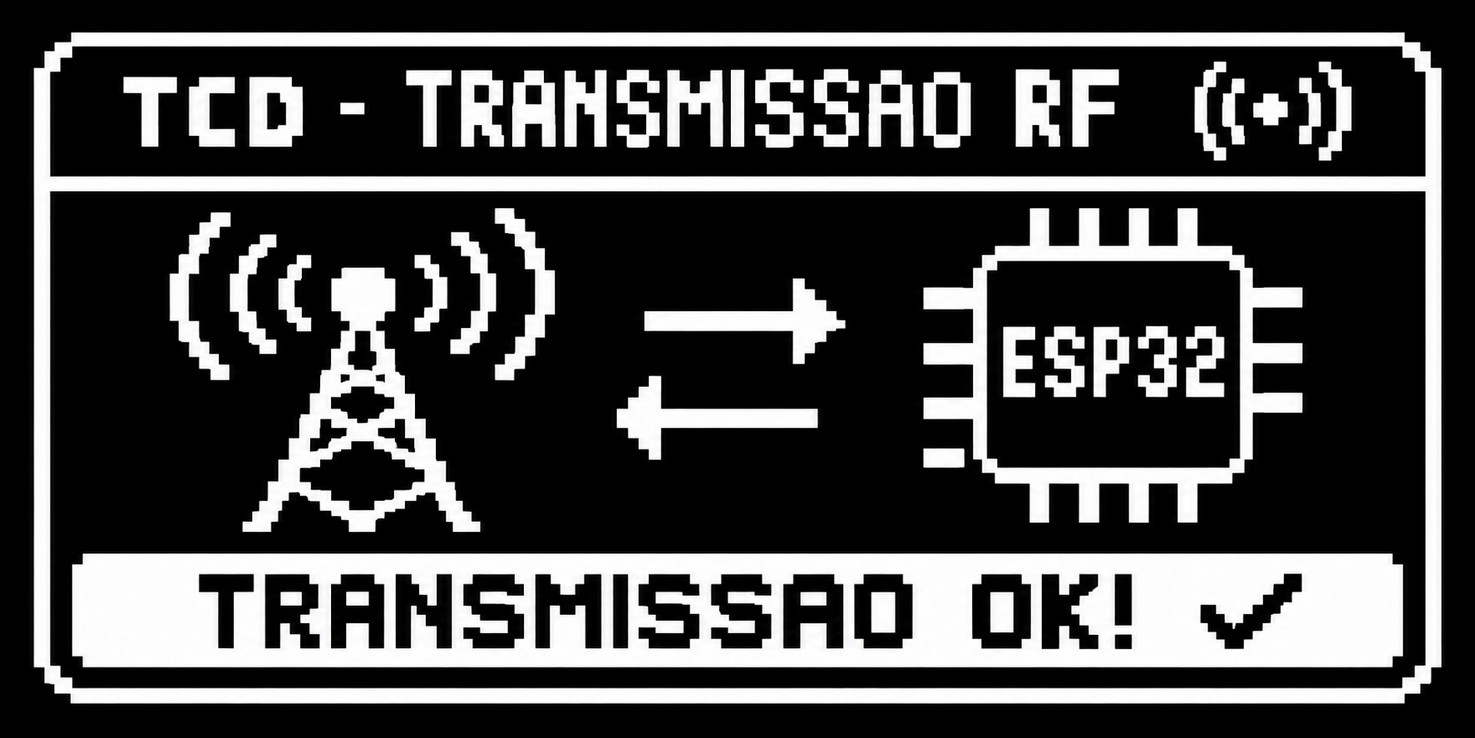
\includegraphics[width=\linewidth,height=145pt,keepaspectratio]{figuras/new_17_1.jpg}\caption{Imagem JPEG de referência utilizada nos ensaios. Fonte: relatório de ensaios, figura 28.}\label{fig:new_17_1}\end{figure}
\setcounter{subsection}{0}\subsection{Passo a passo da transmissão de imagem}
\begin{enumerate}
\item Preparar imagem4.jpeg na pasta em que o script transmissor será executado. Instalar pyserial e Pillow nos dois computadores.
\item Fechar os Monitores Seriais. Conferir a COM atribuída a cada ESP32; uma porta serial não pode ser usada simultaneamente pelo Arduino IDE e pelo script Python.
\item Abrir primeiro o receptor no computador de destino. Para T12 e T13, o receptor foi o B, na COM8.
\item Executar o transmissor no computador de origem. A opção --size seleciona 64\ensuremath{\times}32 ou 128\ensuremath{\times}64. Aguardar a confirmação completa, inclusive END.
\item No destino, conferir o total de bytes, CRC32 e SHA-256 dos pixels. Abrir o PBM/PNG e observar o OLED se o destino for B.
\item Encerrar o receptor antes de inverter o sentido. No T14, A recebeu na COM20 e B enviou pela COM5.
\end{enumerate}
\par\noindent\begin{minipage}{\linewidth}
\begin{lstlisting}
# Receptor B (T12 e T13)
python receber_imagem_TCD.py COM8

# Transmissor A: executar uma resolução por sessão
python enviar_imagem_TCD.py COM20 "imagem4.jpeg" --size 64x32
python enviar_imagem_TCD.py COM20 "imagem4.jpeg" --size 128x64
\end{lstlisting}
\end{minipage}\par
\par\noindent\begin{minipage}{\linewidth}
\begin{lstlisting}
# T14: receptor A; depois transmissor B
python receber_imagem_TCD.py COM20
py enviar_imagem_TCD.py COM5 "imagem4.jpeg" --size 64x32
\end{lstlisting}
\end{minipage}\par
\subsubsection*{Tratamento de falhas observadas}
Se houver erro de acesso à porta COM, fechar programas que a utilizam, verificar o cabo e identificar novamente a porta. Se ocorrerem timeouts sucessivos, registrar o log, encerrar a sessão e diagnosticar primeiro por texto. No T12 houve ClearCommError depois da validação e do salvamento; no T14, a primeira sessão foi interrompida e o envio foi retomado após diagnóstico. Não interpretar uma tentativa interrompida como uma transferência bem-sucedida.

